%FOR PDFLATEX USE ONLY
\documentclass[a4paper,12pt]{article}

\usepackage{amssymb,amsmath} %math symbols

\usepackage[margin=2cm]{geometry} %paper geometry

\usepackage[utf8]{inputenc} %allows unicode (including russian) source file
\usepackage[russian]{babel} %docment in russian-style
\usepackage[utf8]{inputenc}
\usepackage[unicode]{hyperref} %links inside of the text
\usepackage[pdftex]{graphicx} %includegraphics pictures
\usepackage{cmlgc} %bold text

\usepackage{float}

\usepackage{array} %arrays

\usepackage{wrapfig}
\usepackage{array}
\usepackage{lipsum}
\usepackage{esvect}
\usepackage{hyperref}

\usepackage{subfig}
\usepackage{calc}
\usepackage{pgfplots,tikz,circuitikz}
\usepackage{tkz-euclide}

\usepackage{import}
\usepackage{xifthen}
\usepackage{pdfpages}
\usepackage{transparent}

\graphicspath{data/}

\newcommand{\incfig}[1]{%
    \def\svgwidth{\columnwidth}
    \import{./figures/}{#1.pdf_tex}
}

\begin{document}
\begin{titlepage}
    \begin{center}
        {\large МОСКОВСКИЙ ФИЗИКО-ТЕХНИЧЕСКИЙ ИНСТИТУТ (НАЦИОНАЛЬНЫЙ ИССЛЕДОВАТЕЛЬСКИЙ УНИВЕРСИТЕТ)}
    \end{center}
    \begin{center}
        {\largeФизтех-школа прикладной математики и информатики}
    \end{center}

    \vspace{7cm}
    {\huge
        \begin{center}
            {\bf Лабораторная работа 2.5.1}\\
            Измерение коэффициента
            поверхностного натяжения жидкости.
        \end{center}
    }
    \vspace{2cm}
    \begin{flushright}
        {\LARGE Автор:\\ Чикин Андрей \\
            \vspace{0.2cm}
            Б05-304}
    \end{flushright}
    \vspace{3.5cm}
    \begin{center}
        Долгопрудный 2024
    \end{center}
\end{titlepage}

\large
\section{Цель работы:}
1) измерение температурной зависимости  коэффициента поверхностного натяжения дистиллированной воды с использованием известного коэффициента поверхностного натяжения спирта;
\\\\2) определение полной поверхностной энергии  и теплоты, необходимой для изотермического образования единицы  поверхности жидкости  при различной температуре.

\section{В работе используются:}
Прибор  Ребиндера  с термостатом и микроманометром; исследуемые жидкости; стаканы.

\section{Теоретическая часть:}
Из-за поверхностного натяжения возникают разные давления с разных сторон искривленной поверхности жидкости:
\begin{equation}
    \Delta P = P_\text{внутри} - P_\text{снаружи} = \frac{2\sigma}{r} \;\text{(формула Лапласа)}
\end{equation}
$\sigma$ - коэффицент поверхностного натяжения, $r$ - радиус кривизны поверхности.

\section{Экспериментальная установка:}
\begin{figure}[H]
    \center
    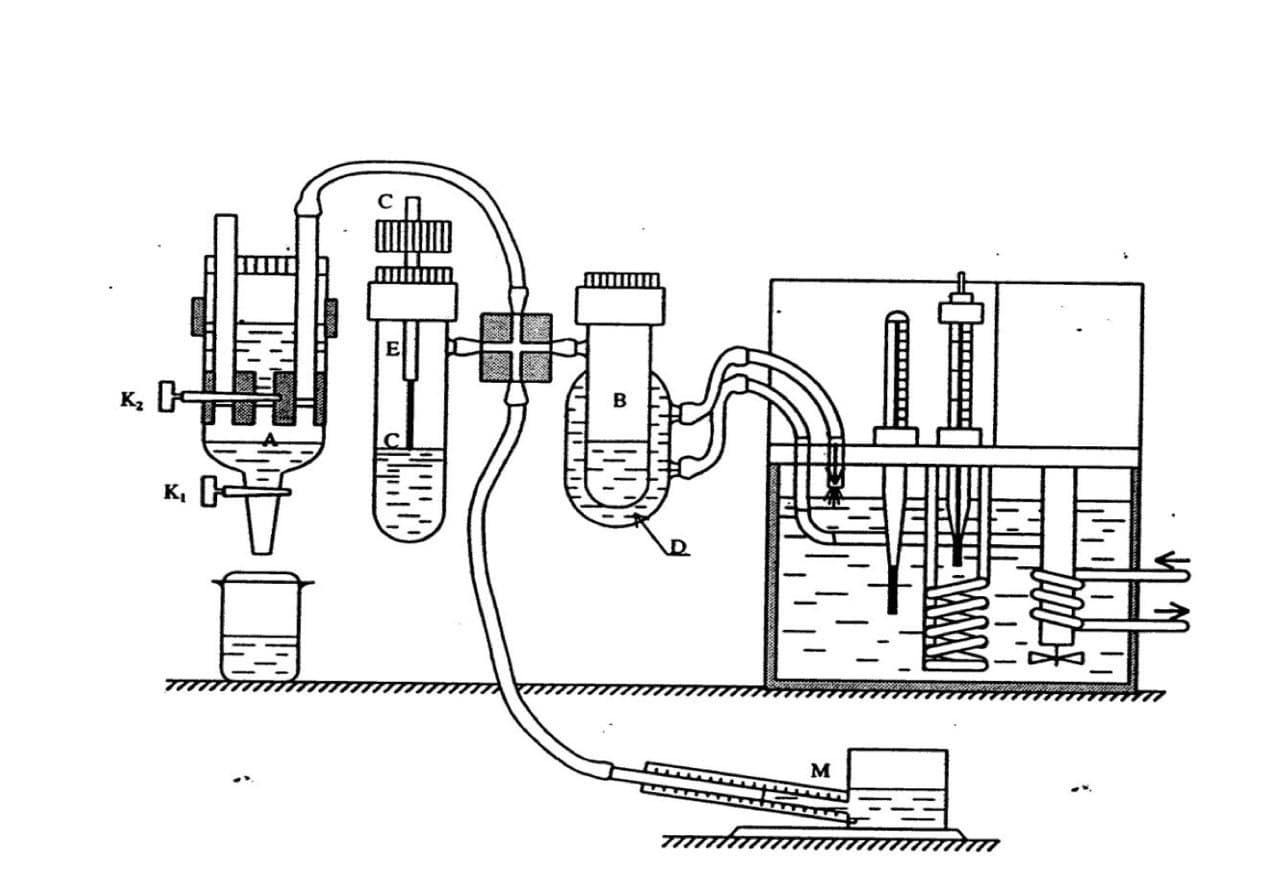
\includegraphics[width=\linewidth]{data/установка.jpg}
    \caption{Схема экспериментальной установки}\label{установка}
\end{figure}
Схема экспериментальной установки представлена на рисунке \ref{установка}.
Тестовая жидкость (этиловый спирт) наливается в сосуд, через пробку в него входит полая металлическа игла. При создании достаточно разреженного воздуха в колбе пузырьки воздуха начинают пробулькивать, поверхностное натяжение измеряется по величине разряжения. Разряжение создается с помощью аспиратора, разность давлений измеряется спиртовым микроманометром.

Для стабилизации температуры через рубашку колбы с исследуемой жидкостью прогоняется вода из термостата. Из-за большой теплопроводности трубки температура в разных частях трубки заметно различна и ввиду теплового расширения поднимается уровень жидкости при изменении температуры. Поэтому при температурном измерениии кончик иглы опускают до самого дна сосуда, тогда:
\begin{equation}
    \Delta P = P - \rho g h
\end{equation}
$\rho$ - плотность жидкости, $h$ - высота погружения иглы.

\section{Измерения и обработка данных}
\subsection*{Измерение радиуса иглы}
Измерение радиусы иглы проводится двумя различными способами: с помощью коэффиента поверхностного натяжения спирта и непосредственно на микроскопе.
При измерении давления нужно умножить показания прибора на $0.2\cdot 9.80665$
Для спирта максимальное давление $\Delta P = 82.38Па$

\begin{table}[h!]
    \caption{Радуис иглы, измеренный через эталонную жидкость (спирт)}
    \label{радиус_спирт}
    \begin{tabular}{|l|l|l|}
        \hline
        r, $10^{-3}$ м & $\sigma_r$,  $10^{-3}$м & $\varepsilon$, \% \\ \hline
        0.55           & 0.009                   & 1.9               \\ \hline
    \end{tabular}
\end{table}

При измерении на микроскопе получается диаметр иглы, равный:
\begin{equation}
    d = (1.10 \pm 0.05 )\ \mili \m
\end{equation}
В дальнейшем примем $d$, равный измеренному микроскопом, так как рехультаты измерений близки друг к другу.

\subsection*{Измерения глубины погружения}
При погружении получаем значение, измеренное линейкой, равное 2.1 см, а перепад давлений равен 93 пункта или 182.4 Па, что соответствует 1.9 см столба воды.

\subsection*{Коэффициент поверхностного натяжения от температуры}

После обработки с известным радиусом иглы и перепадом высот, получим значения коэффицента поверхностного натяжения, представим в виде графика (\ref{sigma})
\begin{figure}[H]
    \begin{center}
        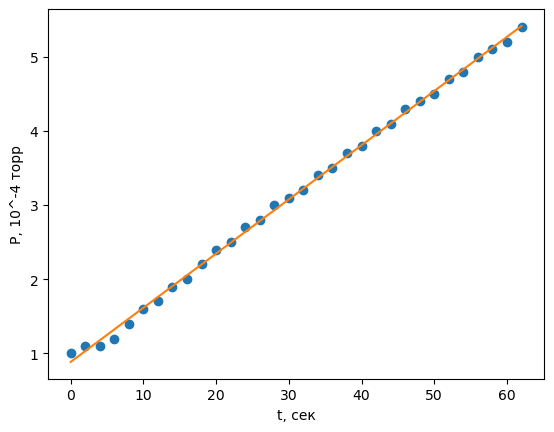
\includegraphics[width=\textwidth]{data/plot1.png}
    \end{center}
    \caption{Зависимость коэффицента поверхностного натяжения воды от температуры} \label{sigma}
\end{figure}
Значения коэффицента натяжения при измерениях на глубине сосуда близки к табличным, их и будем учитывать при дальнейших расчетах. Несовпадение с результами измерений на поверхности жидкости объясняется теплопроводностью металла.

Из аппроксимации графика найдем $\frac{d\sigma}{dt}$, а также построим график теплоты образования единицы поверхности жидкости от температуры и график поверхностной энергии единицы площади.

\begin{table}[H]
    \caption{Зависимость коэффицента поверхностного натяжения воды от температуры}
    \label{dsigma}
    \begin{tabular}{|l|l|l|}
        \hline
        $\frac{d\sigma}{dt}$, $10^{-3}\;   \frac{\text{мН}}{\text{м} \cdot K}$ & $\sigma_\sigma$, $10^{-3}\; \frac{\text{мН}}{\text{м} \cdot K}$ & $\varepsilon$, \% \\ \hline
        -0.129                                                                 & 0.040                                                           & 20                \\ \hline
    \end{tabular}
\end{table}

(\ref{data2})
\begin{figure}[H]
    \begin{center}
        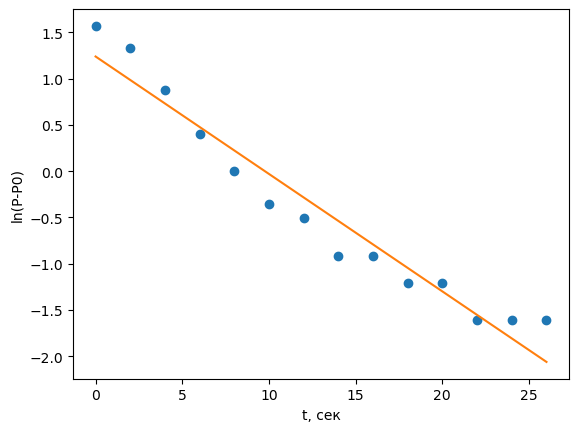
\includegraphics[width=\textwidth]{data/plot2.png}
    \end{center}
    \caption{Теплота образования единицы поверхности жидкости и поверхностная энергия единицы площади} \label{data2}
\end{figure}

(\ref{ass})
\begin{figure}[H]
    \begin{center}
        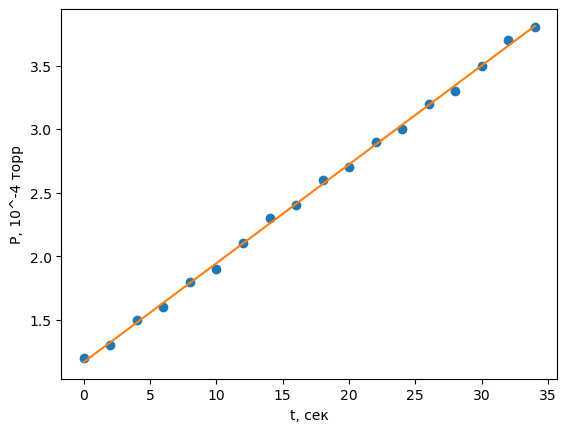
\includegraphics[width=\textwidth]{data/plot3.png}
    \end{center}
    \caption{Зависимость теплоты образования единицы поверхности жидкости от температуры и поверхностной энергии единицы площади} \label{ass}
\end{figure}

\section{Выводы}
\hspace{5mm}
1. Измерены коэффциенты поверхностного натяжения при разных температур, пронаблюдалась близость полученных результатов к табличным значениям.

2. Получена температурная зависимость коэффициента поверхностного натяжения воды от температуры. $\frac{d\sigma}{dt} \;=\; -0.129 \pm 0.040$, $10^{-3}\; \frac{\text{мН}}{\text{м} \cdot K}$ при теоретическом значении $\frac{d\sigma}{dt} = -0.15$, $10^{-3}\; \frac{\text{мН}}{\text{м} \cdot K}$

3. Вычислены зависимости теплоты образования единицы поверхности жидкости от температуры и поверхностной энергии единицы площади, постоянство второй из них подтверждается теоретически.
\end{document}
